\documentclass[10pt,aspectratio=169]{beamer}

% Tema Metropolis moderno
\usetheme{metropolis}
\metroset{progressbar=frametitle, block=fill}

% Paquetes esenciales
\usepackage[spanish,es-nodecimaldot]{babel}
\usepackage[utf8]{inputenc}
\usepackage{amsmath,amssymb,amsfonts}
\usepackage{graphicx}
\usepackage{booktabs}
\usepackage{microtype}

% Directorio de figuras
\graphicspath{{graficas/}}

% Paleta de colores personalizada de alto contraste
\definecolor{NavyDark}{HTML}{0B2545}
\definecolor{NavyMedium}{HTML}{134074}
\definecolor{TealAccent}{HTML}{2A9D8F}
\definecolor{CoralAccent}{HTML}{E63946}
\definecolor{SandLight}{HTML}{F8F9FA}
\definecolor{GrayDark}{HTML}{2B2D42}
\definecolor{PurpleAccent}{HTML}{7A5195}

\setbeamercolor{palette primary}{bg=NavyDark,fg=white}
\setbeamercolor{palette secondary}{bg=NavyMedium,fg=white}
\setbeamercolor{progress bar}{fg=TealAccent,bg=NavyMedium!30}
\setbeamercolor{title separator}{fg=TealAccent}
\setbeamercolor{block title}{bg=NavyMedium,fg=white}
\setbeamercolor{block body}{bg=SandLight,fg=GrayDark}
\setbeamercolor{alerted text}{fg=CoralAccent}

% Título y Metadatos
\title{Autopsia de una Red Neuronal}
\subtitle{¿Qué Aprende Realmente la IA Cuando Nadie la Vigila?}
\author{\textbf{Laboratorio de Inteligencia Artificial} --- Sesión Magistral de Interpretabilidad}
\date{\today}
\institute{Deep Learning, Diagnóstico Forense y Límites de la IA}

\begin{document}

% -----------------------------------------------------------------------------
% SLIDE 1: PORTADA
% -----------------------------------------------------------------------------
\begin{frame}
  \titlepage
\end{frame}

% -----------------------------------------------------------------------------
% SLIDE 2: PRÓLOGO — HOY NADIE DERIVA NADA
% -----------------------------------------------------------------------------
\begin{frame}{Prólogo: Hoy Nadie Deriva Nada}
  \begin{columns}[T]
    \begin{column}{0.48\textwidth}
      \begin{block}{Lo que ya conquistamos}
        \scriptsize
        En las sesiones previas construimos el pipeline completo:
        \begin{itemize}
          \item Backpropagation y optimización con Adam.
          \item Curvas de aprendizaje y diagnóstico de sobreajuste.
          \item Parada temprana (\textit{Early Stopping}) y checkpoints en disco (\texttt{mejor\_modelo.pth}).
        \end{itemize}
      \end{block}

      \vspace{-0.1cm}
      \begin{block}{El Cambio de Rol Hoy}
        \scriptsize
        Hoy colgamos el traje de programadores matemáticos y nos ponemos la bata de \textbf{detectives forenses}.
      \end{block}
    \end{column}

    \begin{column}{0.48\textwidth}
      \begin{alertblock}{La Pregunta Incómoda}
        \scriptsize
        \begin{center}
          \textit{«El modelo entrenó sin errores y la pérdida bajó... \\ pero ¿realmente aprendió economía de demanda, o solo encontró una trampa para engañarnos?»}
        \end{center}
      \end{alertblock}

      \vspace{0.1cm}
      \textbf{La Agenda de Hoy}:
      \begin{enumerate}\scriptsize
        \item \textbf{Acto 1}: Los peores fallos reales de nuestra red.
        \item \textbf{Acto 2}: El efecto Clever Hans (lobos, nieve y rayos X).
        \item \textbf{Acto 3}: La trampa de la extrapolación.
        \item \textbf{Acto 4}: El mapa del zoológico de la IA.
      \end{enumerate}
    \end{column}
  \end{columns}
\end{frame}

% -----------------------------------------------------------------------------
% SLIDE 3: ACTO 1 — LA AUTOPSIA FORENSE DE NUESTRO MODELO
% -----------------------------------------------------------------------------
\begin{frame}{Acto 1: La Autopsia Forense de Nuestro Modelo}
  \begin{columns}[c]
    \begin{column}{0.54\textwidth}
      \begin{center}
        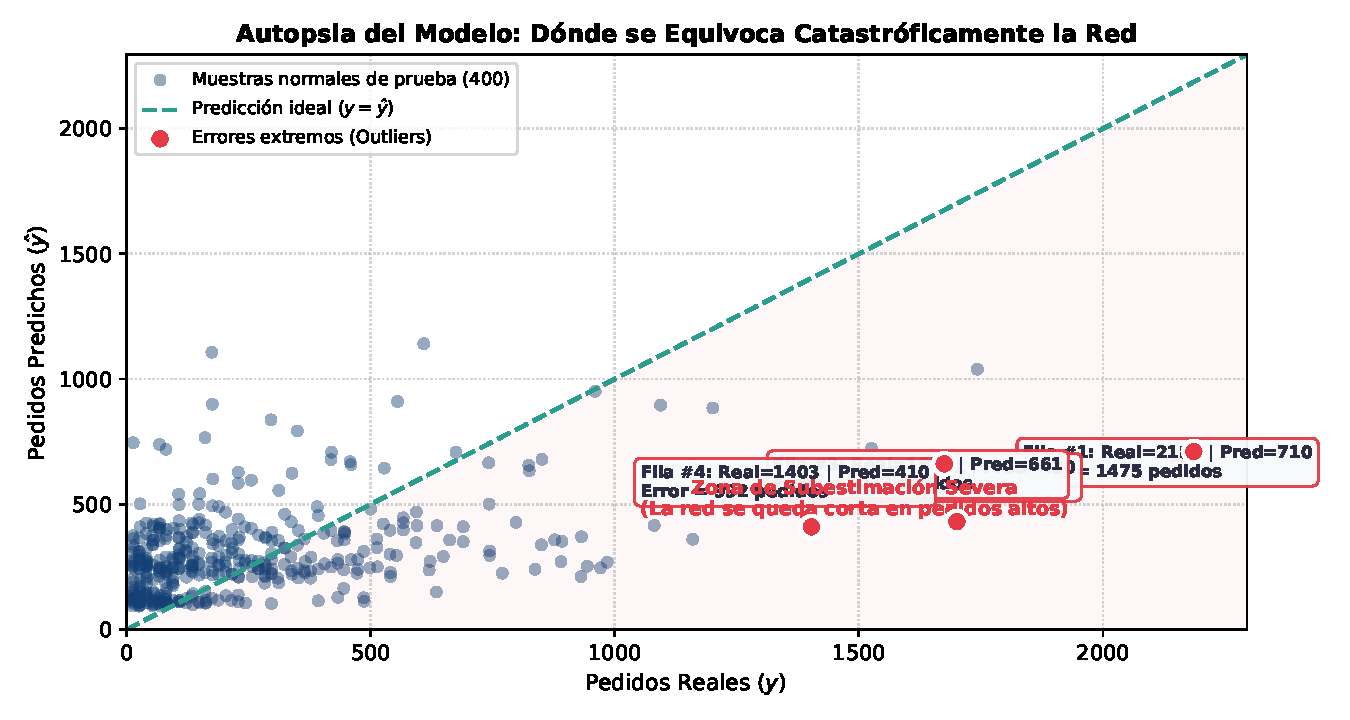
\includegraphics[width=\linewidth]{autopsia_peores_errores.pdf}
      \end{center}
    \end{column}

    \begin{column}{0.44\textwidth}
      \textbf{Los Datos No Mienten (\texttt{predicciones\_prueba.csv})}:
      \vspace{0.15cm}

      \scriptsize
      \begin{tabular}{r r r}
        \toprule
        \textbf{Real ($y$)} & \textbf{Predicho ($\hat{y}$)} & \textbf{Error Absoluto} \\
        \midrule
        \textbf{1,701} & 431 & \alert{\textbf{1,270 pedidos}} \\
        \textbf{944}   & 253 & \alert{\textbf{691 pedidos}} \\
        \textbf{770}   & 225 & \alert{\textbf{545 pedidos}} \\
        161   & \textbf{766} & \alert{\textbf{605 pedidos}} \\
        \bottomrule
      \end{tabular}

      \vspace{0.25cm}
      \textbf{El Patrón Detectado}:
      \begin{itemize}\scriptsize
        \item Cuando la demanda explota ($> 900$), la red \textbf{colapsa hacia abajo}.
        \item Predice tímidamente entre $200$ y $450$ pedidos.
        \item ¿Por qué una red con $241$ pesos comete este error sistemático?
      \end{itemize}
    \end{column}
  \end{columns}
\end{frame}

% -----------------------------------------------------------------------------
% SLIDE 4: LA TRAMPA DEL PROMEDIO Y EL ERROR CUADRÁTICO
% -----------------------------------------------------------------------------
\begin{frame}{¿Por qué Falló la Red? La Trampa de la Pérdida Cuadrática}
  \begin{columns}[T]
    \begin{column}{0.48\textwidth}
      \begin{block}{La Matemática Detrás de la Cobardía}
        \scriptsize
        Nuestra función de pérdida fue el Error Cuadrático Medio:
        \[
          \mathcal{L}_{\text{MSE}} = \frac{1}{N} \sum_{i=1}^N (y_i - \hat{y}_i)^2
        \]
        \begin{itemize}
          \item En el dataset, el $95\%$ de las semanas tienen entre $50$ y $350$ pedidos (promedio real: $258$).
          \item Si la red se arriesga a predecir $1,500$ pedidos y esa semana solo hubo $200$, el error cuadrático es:
          \[
            (1,500 - 200)^2 = 1,690,000 \quad \text{\alert{(Pena capital)}}
          \]
          \item La red descubrió que \textbf{apostar al promedio} es la estrategia más segura para mantener el gradiente bajo control.
        \end{itemize}
      \end{block}
    \end{column}

    \begin{column}{0.48\textwidth}
      \begin{alertblock}{La Primera Gran Lección}
        \scriptsize
        \textbf{La red no es tonta, es obediente}:
        \begin{itemize}
          \item Optimizó a la perfección la función matemática que nosotros le dimos.
          \item Si le pides minimizar $(y - \hat{y})^2$, sacrificará la precisión en los días extraordinarios para protegerse en los días ordinarios.
          \item \textbf{Solución de ingeniería}: Transformación logarítmica $\log(1 + y)$ o función Huber Loss en problemas asimétricos.
        \end{itemize}
      \end{alertblock}
    \end{column}
  \end{columns}
\end{frame}

% -----------------------------------------------------------------------------
% SLIDE 5: ACTO 2 — EL EFECTO CLEVER HANS EN MACHINE LEARNING
% -----------------------------------------------------------------------------
\begin{frame}{Acto 2: El Fenómeno ``Clever Hans'' en Machine Learning}
  \begin{columns}[T]
    \begin{column}{0.48\textwidth}
      \begin{block}{Alemania, 1904: El Caballo Sabio}
        \scriptsize
        \textbf{Clever Hans} era un caballo que supuestamente sabía sumar, restar y multiplicar:
        \begin{itemize}
          \item Su dueño le preguntaba: \textit{«¿Cuánto es $3 + 2$?»}
          \item El caballo golpeaba el suelo con el casco $5$ veces y se detenía.
          \item Científicos de toda Europa viajaron a certificar el ``milagro''.
        \end{itemize}
      \end{block}

      \vspace{-0.1cm}
      \begin{block}{El Experimento del Dr. Oskar Pfungst}
        \scriptsize
        Pfungst aisló al caballo del público y del dueño:
        \begin{itemize}
          \item El caballo \textbf{falló por completo}.
          \item Descubrimiento: Hans no sabía aritmética; leía la tensión en las cejas y respiración del público cuando llegaba al número correcto.
        \end{itemize}
      \end{block}
    \end{column}

    \begin{column}{0.48\textwidth}
      \begin{alertblock}{El Paralelismo con Deep Learning}
        \scriptsize
        \begin{itemize}
          \item Las redes neuronales son los \textbf{Clever Hans modernos}.
          \item No comprenden conceptos semánticos ni causas físicas.
          \item Son máquinas estadísticas implacables que explotarán \textbf{cualquier atajo accidental (\textit{shortcut})} en los datos con tal de bajar la pérdida.
        \end{itemize}
      \end{alertblock}
    \end{column}
  \end{columns}
\end{frame}

% -----------------------------------------------------------------------------
% SLIDE 6: CASO DE ESTUDIO 1 — EL LOBO Y LA NIEVE
% -----------------------------------------------------------------------------
\begin{frame}{Caso de Estudio 1: El Lobo y la Nieve (Fotos Reales)}
  \begin{columns}[T]
    \begin{column}{0.54\textwidth}
      \begin{center}
        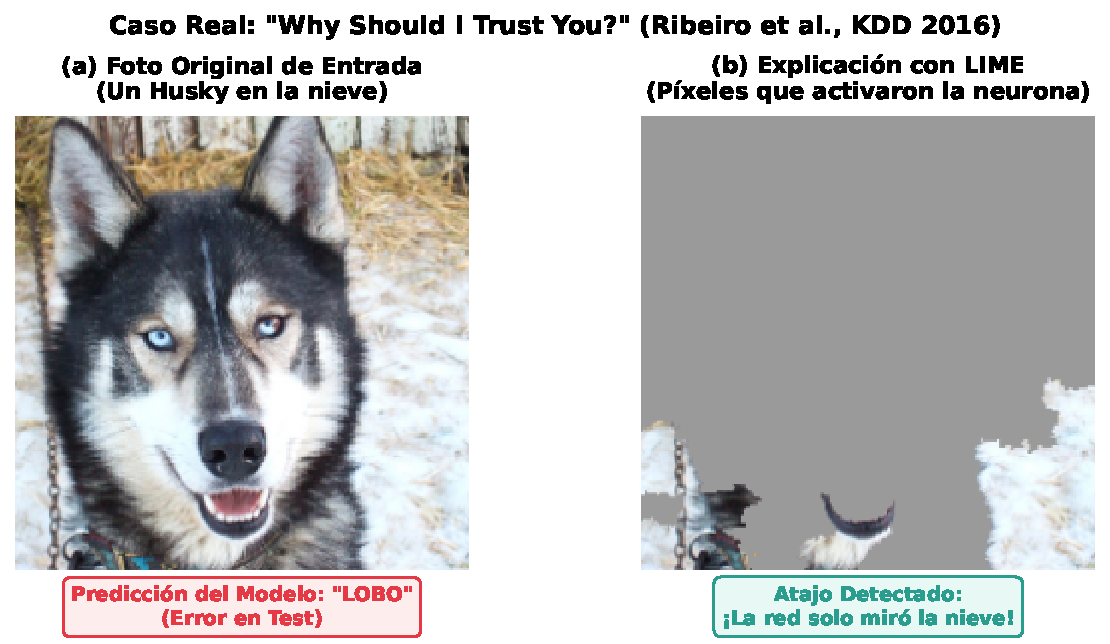
\includegraphics[width=\linewidth,height=0.68\textheight,keepaspectratio]{clever_hans_lobo_nieve_real.pdf}
      \end{center}
    \end{column}

    \begin{column}{0.44\textwidth}
      \begin{block}{El Paper Seminal de LIME (2016)}
        \scriptsize
        Ribeiro et al. entrenaron una red profunda para \textbf{Lobos vs. Huskies}:
        \begin{itemize}
          \item Precisión casi perfecta en test ($>95\%$).
          \item Ante este husky real, predijo \alert{\textbf{``LOBO''}} con total seguridad.
        \end{itemize}
      \end{block}

      \vspace{-0.15cm}
      \begin{alertblock}{La Autopsia de Píxeles}
        \scriptsize
        Al aplicar LIME para ver qué activó la neurona:
        \begin{itemize}
          \item El perro fue \textbf{ignorado por completo}.
          \item La decisión se basó exclusivamente en la \textbf{nieve blanca del fondo}.
          \item \textit{Conclusión}: La red jamás aprendió animales; aprendió un detector de nieve.
        \end{itemize}
      \end{alertblock}
    \end{column}
  \end{columns}
\end{frame}

% -----------------------------------------------------------------------------
% SLIDE 7: CASO DE ESTUDIO 2 — RAYOS X DE COVID Y MARCAS DE AGUA
% -----------------------------------------------------------------------------
\begin{frame}{Caso de Estudio 2: Radiografías de COVID y la Letra de Metal}
  \begin{columns}[T]
    \begin{column}{0.48\textwidth}
      \begin{block}{El Desafío Clínico de 2020}
        \scriptsize
        Durante el pico de la pandemia se publicaron cientos de modelos de Deep Learning que prometían detectar COVID-19 en radiografías de tórax con $95\%+$ de sensibilidad:
        \begin{itemize}
          \item Se entrenaron con radiografías de decenas de hospitales del mundo.
          \item Parecía un triunfo absoluto de la inteligencia artificial médica.
        \end{itemize}
      \end{block}

      \vspace{-0.15cm}
      \begin{block}{La Autopsia Científica (Nature, 2021)}
        \scriptsize
        Científicos de Cambridge auditaron más de $400$ modelos y descubrieron que \textbf{ninguno servía en clínica}:
        \begin{itemize}
          \item Los pacientes graves en UCI se escaneaban con equipos portátiles que dejaban una pequeña letra ``R'' metálica o tipografías distintas.
        \end{itemize}
      \end{block}
    \end{column}

    \begin{column}{0.48\textwidth}
      \begin{alertblock}{El Atajo Mortal}
        \scriptsize
        \begin{center}
          La red neuronal aprendió a clasificar: \\
          \vspace{0.15cm}
          \textbf{¿Qué máquina de rayos X tomó la foto?} \\
          en vez de \\
          \textbf{¿El pulmón tiene neumonía?}
        \end{center}
        \vspace{0.1cm}
        Al llevar el modelo a un hospital nuevo sin esas marcas, la precisión cayó al azar ($50\%$).
      \end{alertblock}
    \end{column}
  \end{columns}
\end{frame}

% -----------------------------------------------------------------------------
% SLIDE 8: ACTO 3 — ¿POR QUÉ LA RED NO RAZONA? INTERPOLAR vs EXTRAPOLAR
% -----------------------------------------------------------------------------
\begin{frame}{Acto 3: ¿Por qué la Red no Razona? Interpolar vs. Extrapolar}
  \begin{columns}[c]
    \begin{column}{0.54\textwidth}
      \begin{center}
        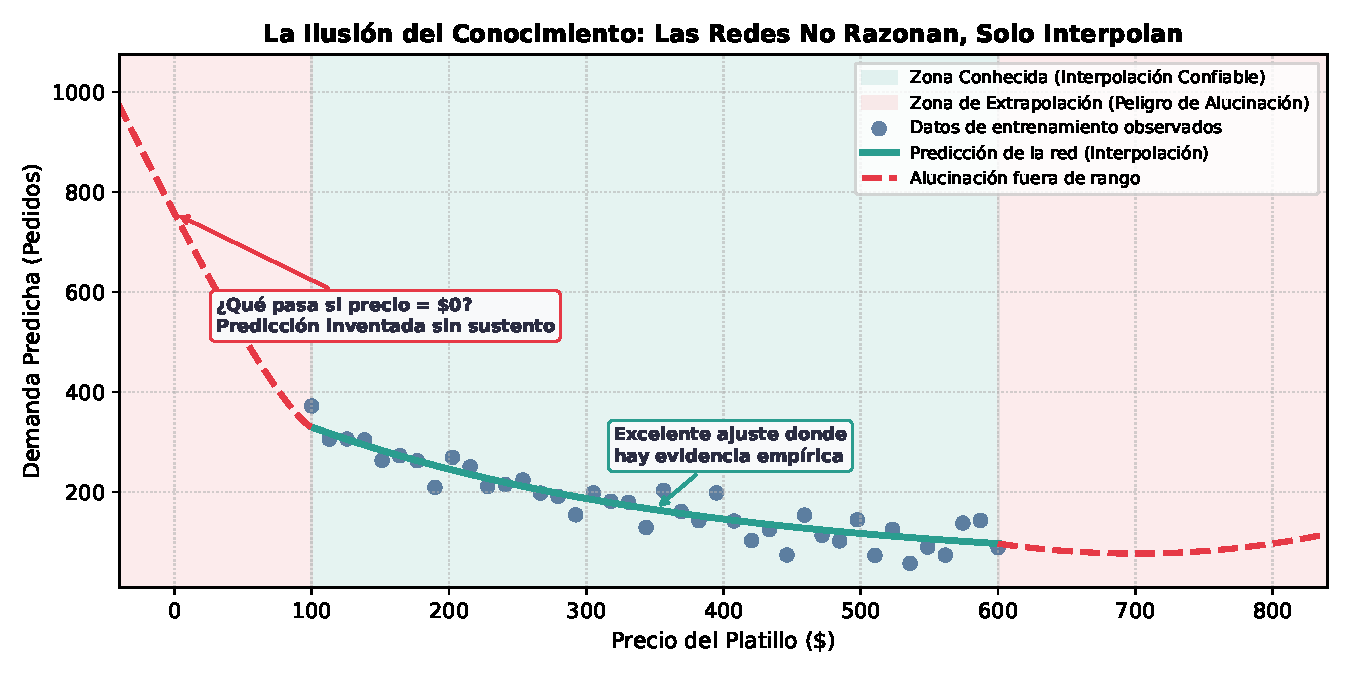
\includegraphics[width=\linewidth]{interpolacion_vs_extrapolacion.pdf}
      \end{center}
    \end{column}

    \begin{column}{0.44\textwidth}
      \begin{block}{La Metáfora de la Sábana de Goma}
        \scriptsize
        Una red neuronal es como una sábana elástica en alta dimensión:
        \begin{itemize}
          \item \textbf{Interpolación (Dentro del dominio)}:
          La sábana se dobla con gracia para tocar todos los puntos observados. Aquí la red es excelente.
          \item \textbf{Extrapolación (Fuera del dominio)}:
          Fuera de los postes donde clavamos los datos, la sábana ondea en cualquier dirección impredecible.
        \end{itemize}
      \end{block}

      \vspace{-0.1cm}
      \begin{alertblock}{La Regla de Oro}
        \scriptsize
        Las redes neuronales \textbf{nunca te dirán «no sé»}.
        Ante una entrada delirante, te responderán un número absurdo con $100\%$ de seguridad numérica.
      \end{alertblock}
    \end{column}
  \end{columns}
\end{frame}

% -----------------------------------------------------------------------------
% SLIDE 9: EXPERIMENTO DE ESTRÉS CON NUESTRO MODELO
% -----------------------------------------------------------------------------
\begin{frame}{Experimento de Estrés (\textit{Stress Testing}) con Nuestro Modelo}
  ¿Qué responde \texttt{mejor\_modelo.pth} si le hacemos preguntas fuera de su universo?
  \vspace{0.2cm}

  \begin{center}
    \scriptsize
    \begin{tabular}{p{3.2cm} p{3.2cm} p{5.0cm}}
      \toprule
      \textbf{Pregunta al Modelo} & \textbf{Lógica Económica Real} & \textbf{Comportamiento de la Red} \\
      \midrule
      Precio = \textbf{\$0.00} (Comida gratis) &
      Demanda infinita / colapso de inventario &
      Predice un valor finito arbitrario ($\sim 500$ pedidos) porque jamás vio un precio menor a $\$130$. \\
      \addlinespace
      Precio = \textbf{\$100,000.00} (Precio astronómico) &
      Demanda exactamente $0$ &
      Predice números positivos absurdos debido a la saturación de las capas lineales. \\
      \addlinespace
      Semana = \textbf{999} (20 años en el futuro) &
      Incertidumbre total &
      Extrapola linealmente el peso asignado a \texttt{week}, disparando la predicción sin control. \\
      \bottomrule
    \end{tabular}
  \end{center}

  \vspace{0.2cm}
  \begin{block}{Conclusión de la Prueba de Estrés}
    \scriptsize
    El modelo carece de sentido común. No sabe qué es el dinero, qué es el apetito ni qué es una semana. Solo calcula $\sigma(Wx + b)$.
  \end{block}
\end{frame}

% -----------------------------------------------------------------------------
% SLIDE 10: INGENIERÍA DE MITIGACIÓN — ENJAULAR A LA BESTIA
% -----------------------------------------------------------------------------
\begin{frame}{Ingeniería de Mitigación: Enjaular a la Bestia en Producción}
  En la industria seria, una red neuronal \textbf{jamás se conecta directamente al cliente sin blindaje}:
  \vspace{0.15cm}

  \begin{columns}[T]
    \begin{column}{0.32\textwidth}
      \begin{block}{1. Vallas de Entrada (\textit{Guardrails})}
        \scriptsize
        Validar el dominio antes de tocar la red:
        \begin{itemize}
          \item \texttt{assert 100 <= precio <= 800}
          \item Si el dato está fuera, rechazar o recortar al percentil permitido (\textit{clipping}).
        \end{itemize}
      \end{block}
    \end{column}

    \begin{column}{0.34\textwidth}
      \begin{block}{2. Reglas Fijas de Negocio}
        \scriptsize
        Combinar IA con lógica determinista:
        \begin{itemize}
          \item «Si precio es cero, no consultes a la red; activa protocolo de promoción gratuita».
          \item La IA asesora; el código duro manda.
        \end{itemize}
      \end{block}
    \end{column}

    \begin{column}{0.32\textwidth}
      \begin{block}{3. Detección OOD (\textit{Out-of-Distribution})}
        \scriptsize
        Calcular la distancia de Mahalanobis:
        \begin{itemize}
          \item ¿Este cliente se parece a los datos históricos?
          \item Si la distancia es alta $\implies$ encender alarma de baja confianza.
        \end{itemize}
      \end{block}
    \end{column}
  \end{columns}
\end{frame}

% -----------------------------------------------------------------------------
% SLIDE 11: ACTO 4 — EL ZOOLÓGICO DE LA IA (HACIA DÓNDE VAMOS)
% -----------------------------------------------------------------------------
\begin{frame}{Acto 4: El Zoológico de la IA (Hacia Dónde Vamos)}
  \begin{center}
    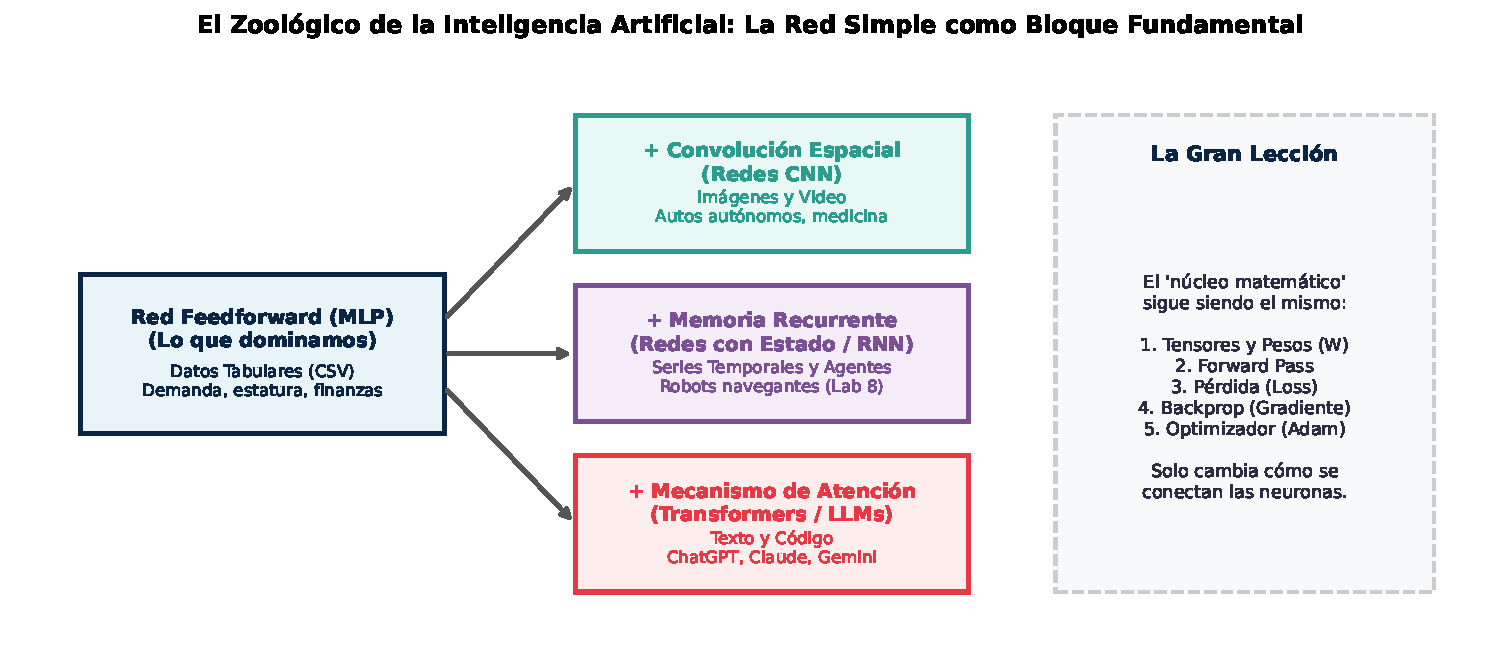
\includegraphics[width=0.78\textwidth,height=0.46\textheight,keepaspectratio]{mapa_zoologico_ia.pdf}
  \end{center}
  \vspace{-0.25cm}
  \begin{columns}[T]
    \begin{column}{0.48\textwidth}
      \textbf{Lo que Ya Dominas}:
      \begin{itemize}\scriptsize
        \item Red densa feedforward (MLP) para tablas y números continuos.
        \item Entendiste el ciclo completo: Datos $\to$ Tensores $\to$ Pérdida $\to$ Gradiente $\to$ Checkpoint.
      \end{itemize}
    \end{column}
    \begin{column}{0.48\textwidth}
      \textbf{La Conexión con los Próximos Temas}:
      \begin{itemize}\scriptsize
        \item Para imágenes: añadiremos \textbf{convoluciones} (CNNs).
        \item Para secuencias y navegación de robots: añadiremos \textbf{memoria temporal} (como en el Lab 8 del robot).
      \end{itemize}
    \end{column}
  \end{columns}
\end{frame}

% -----------------------------------------------------------------------------
% SLIDE 12: LAS CUATRO REGLAS DE ORO DEL INGENIERO DE IA
% -----------------------------------------------------------------------------
\begin{frame}{Las Cuatro Reglas de Oro del Ingeniero de IA}
  \begin{columns}[T]
    \begin{column}{0.48\textwidth}
      \begin{block}{1. La Métrica Única es una Ilusión}
        \scriptsize
        Tener un $R^2$ decente o un $98\%$ de precisión no significa nada si no abres la gráfica de residuos y miras los casos individuales donde el modelo falló.
      \end{block}

      \vspace{-0.1cm}
      \begin{block}{2. La Red Siempre Hará Trampa}
        \scriptsize
        Si hay una correlación espuria (nieve, marcas de agua, orden temporal), el optimizador la aprenderá antes que el concepto real.
      \end{block}
    \end{column}

    \begin{column}{0.48\textwidth}
      \begin{block}{3. Conoce las Fronteras de tu Sábana}
        \scriptsize
        El modelo solo es dueño del espacio donde tiene datos. Fuera de ahí, no es inteligencia artificial: es generación aleatoria de números con arrogancia matemática.
      \end{block}

      \vspace{-0.1cm}
      \begin{alertblock}{4. Tu Valor no es Tunear el Learning Rate}
        \scriptsize
        Cualquiera puede correr \texttt{optimizer.step()}. El verdadero ingeniero es quien sabe cuándo el modelo está mintiendo y cómo proteger el sistema real.
      \end{alertblock}
    \end{column}
  \end{columns}
\end{frame}

% -----------------------------------------------------------------------------
% SLIDE 13: CIERRE
% -----------------------------------------------------------------------------
\begin{frame}[standout]
  \Huge ¿Preguntas o Comentarios?
  \vspace{0.4cm}

  \normalsize Pueden dejar sus reflexiones en el chat: \\
  \textit{¿Cuál caso de fallo de IA les pareció más peligroso o curioso?}
\end{frame}

\end{document}
